% Chapter Template

\chapter{Non-thermal emission from \ac{BNS} mergers} \label{ch:afterglow} 

%In this chapter we discuss models of the non-thermal counterpart 
%of the \ac{BNS} mergers, the \ac{kN} afterglow.

In Sec.~\ref{sec:intro:afterglow} we discussed the origin of 
a non-thermal emission from \ac{BNS} mergers, focusing on 
\ac{GRB} and \ac{kN} afterglows. 
%
In this chapter we expand upon this discussion. First, in 
Sec.~\ref{sec:intro:afterglow_modelling}, we recall the basic methods 
of computing the synchrotron emission from a relativistic \blast{} 
expanding into \ac{ISM}. 
%
Then, in Sec.~\ref{sec:afterglow:code}, we describe specific methods 
that we implemented numerically in \pyblast{} code, and verify the 
code performance by comparing our results with published ones. 
%
Finally, in Sec.~\ref{sec:afterglow:results}, we present our results, 
comparing them with observations. 


%% =============================================================
%%
%% P H Y S I C S 
%%
%% =============================================================

\section{Overview of the afterglow modeling methods}\label{sec:intro:afterglow_modelling}

The theory of relativist shocks with applications to \acp{AGN} jets was 
developed by \citet{Blandford:1976}. Later, the theory was successfully 
applied to \ac{GRB} afterglows \citep{Costa:1997cg,vanParadijs:1997wr,Frail:1997qf},
and \ac{kN} afterglows \citep[\eg][]{Nakar:2011cw,Hotokezaka:2015eja,Hotokezaka:2018gmo}.

A way to compute the non-thermal emission from an expanding \blast{} 
is to perform multidimensional 
radiation transport \ac{HD} or \ac{MHD} simulation. However, this 
approach is numerically very expensive due to broad spatial and 
time ranges involved. 
%
It is possible, however, to approximate the \blast{} evolution  
with a semi-analytic one-zone model, neglecting the internal structure 
of the \blast{} \citep{Nava:2013,Peer:2012,Kumar:2014upa}. 
%
%When computing the afterglow emission from the structured relativistic 
%(mildly relativistic) source, 
The key component of afterglow modeling are (i) \blast{} dynamics, 
(ii) electron energy distribution (iii) synchrotron emission. 



\subsection{Dynamical evolution of a \blast{}}

A universal part of the afterglow theory is the dynamics of the \trans{} 
\blast{} propagating through the \ac{ISM}, that is also called ``fireball''.

Analytical studies and numerical simulations showed that an 
expanding into \ac{ISM} a \blast{} generates a pair of shocks: a forward shock, that 
propagates through the upstream \ac{ISM}, and a reverse shock that moves black, 
through the \blast{} \citep[\eg][]{Blandford:1976}. 
%%
\begin{figure*}[t]
    \centering 
    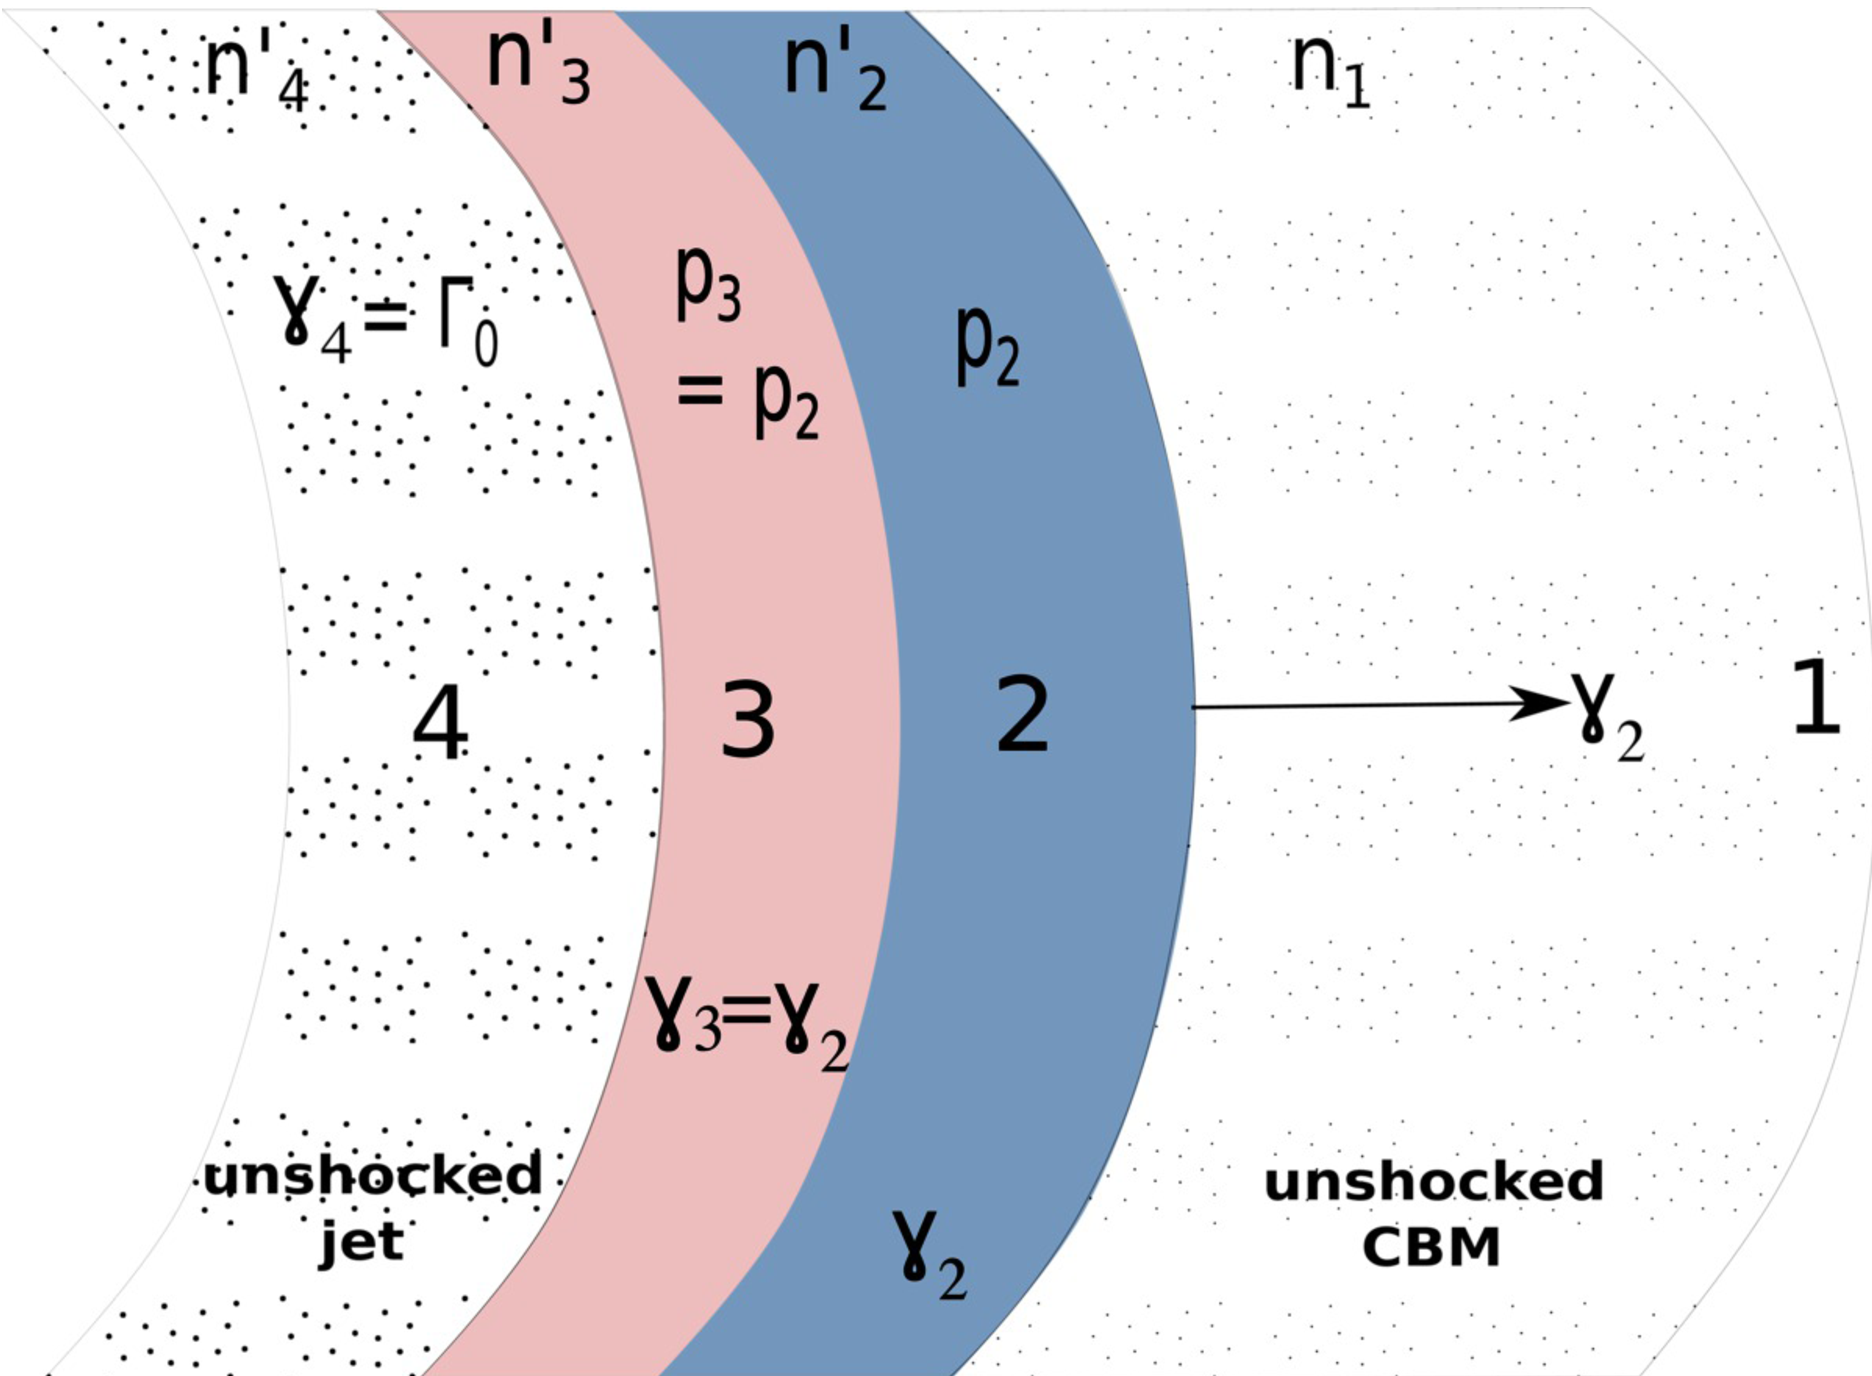
\includegraphics[width=0.45\textwidth]{Fig_8_KZ.pdf}
    \caption{
        This is a schematic sketch of a pair of shocks produced when a relativistic
        jet from a \ac{GRB} collides with the \ac{CBM}, as viewed from the
        rest frame of unshocked \ac{CBM}. Regions 2 \& 3 represent shocked \ac{CBM} and \ac{GRB}
        jet respectively. They move together with the same \ac{LF} ($\gamma_2$, as viewed
        by a stationary observer in the unshocked \ac{CBM}), and have the same pressure but
        different densities.
        (Adapted from \citet{Kumar:2014upa}, Fig.~8)
    }
    \label{fig:aafg:theory:sr8}
\end{figure*}
%%
In Fig.~\ref{fig:aafg:theory:sr8}, this pair of shocks is schematically depicted as 
boundaries between regions $1-2$ and $3-4$ respectively. 
Overall, there are four district regions: unshocked and shocked \ac{ISM} (regions $1$ and $2$), 
and shocked and unshocked \ac{GRB} or \ac{kN} ejecta (regions $3$ and $4$).
The comoving- and observer-frame quantities are marked with and without a superscript prime ($'$) 
respectively. 

The evolution of physical properties of a shock is governed by three conservation laws: 
baryon number, $n' \Gamma c$, and energy and momentum fluxes across the shock front. 
The latter two are a embedded into the fluid energy momentum tensor, Eq.~\eqref{eq:theory:tmunu_perf}. 

Neglecting the internal structure of the \blast{} it is possible to express 
these conservation laws as \citep{Blandford:1976,Rezzolla:2013} 
%%
\begin{equation}
\frac{e_2'}{n_2'} = (\gamma_{21} - 1)m_p c^2, \hspace{5mm}
\frac{n_2'}{n_1'} = \frac{\hat{\gamma}\gamma_{21} + 1}{\hat{\gamma}-1}, \hspace{5mm}
\gamma_{1s}^2 = \frac{(\gamma_{21} + 1) [\hat{\gamma}(\gamma_{21}-1)+1]^2}{\hat{\gamma}(2-\hat{\gamma})(\gamma_{21}-1)+2},
\label{eq:afterglow:blast}
\end{equation}
%%
where subscripts $2$ and $1$ stand for downstream and upstream respectively, 
shown in Fig.~\ref{fig:aafg:theory:sr8}, 
$e'$ is the internal energy density, $n'$ is the proton number density, 
$\gamma_{21}$ is the relative \ac{LF} of plasma in region 
$2$ with respect to the region $1$
$\gamma_{1s}$ is the relative \ac{LF} of plasma in region $1$ with respect to the shock front,
$\hat{\gamma}$ is the adiabatic index of the fluid, which is $\hat{\gamma}=4/3$ 
for the ideal relativistic fluid and $\hat{\gamma}=5/3$ for subrelativisitc fluid.

Solving the system Eq.~\eqref{eq:afterglow:blast} for the 
forward and reverse shocks gives the full evolution of the \blast{}. 

A shock propagating through \ac{ISM} compresses it. For a relativistic case with $\hat{\gamma}=4/3$
$n_2'/n_1' = 3 ((4/3)\gamma_{21} + 1) = 4\gamma_{21} + 3 \approx 4 \gamma_{21}$, 
\ie, the downstream plasma is compressed with compression ratio $4\gamma_{21}$.
%
Additionally, a shock front randomizes the velocity vectors,
of particle, protons, raising their thermal energy, while their \ac{LF} remains
unchanged.


\subsection{Electron distribution}

As the shock compresses the fluid and amplifies random magnetic fields, it accelerates the 
inbound particles to a power-law distribution function. 

The electron distribution function, $dn/d\gamma_e$, can be obtained from 
the continuity equation for electrons in the energy space 
%
\begin{equation}
\label{eq:intro:electron_dist_cont_eq}
\frac{\partial }{\partial t}\frac{d n_e}{d\gamma_e} + \frac{\partial}{\partial \gamma_e}\Big[ \dot{\gamma_e}\frac{dn_e}{d\gamma_e} \Big] = S(\gamma_e)\, ,
\end{equation}
%
where $\dot{\gamma_e} = -\sigma_T B^2 \gamma_e^2 / (6\pi m_e c)$ is the rate at 
which electron \ac{LF} changes due to energy losses, $S(\gamma_e)$ is the injection 
rate of electrons into the system.


Assuming that the injection of electrons is constant (steady-state solution,
$\partial_t = 0$), and has a minimum, $\gamma_m$, such that, 
$S(\gamma_e) = 0$ for $\gamma_e < \gamma_m$, the solutions to the Eq.~\eqref{eq:intro:electron_dist_cont_eq} reads 
%
\begin{equation}
\frac{dn_e}{d\gamma_e} \propto 
\begin{cases}
\gamma_e^{-2} &\text{ if } \gamma_c < \gamma_e < \gamma_m, \\
\gamma_e^{-p-1} &\text{ if } \gamma_e > \gamma_c > \gamma_m
\end{cases}
\label{eq:afterglow:elec_dist}
\end{equation}
%
where $\gamma_c$ is the cooling \ac{LF}, above which electrons loose their 
energy to radiation efficiently over a certain characteristic time.
%
The $\gamma_c < \gamma_e < \gamma_m$ regime is usually referred as 
\textit{slow cooling} and $\gamma_e > \gamma_c > \gamma_m$ as \textit{fast cooling} 
\citep{Sari:1997qe}.



\subsubsection{Synchrotron emission}

The power of the synchrotron radiation, $P'_{syn}$, emitted by an electron moving with 
the speed, $\upsilon_e$, corresponding to the \ac{LF}, $\gamma_e$, 
in the magnetic field, $B$, perpendicular to the field lines is given by the Larmor's formula.
%
As within the magnetic field, an electron is following the spiral trajectory,
the characteristic frequency of the synchtrontron radiation, $\nu'_{syn}$, is given 
by the angular speed of the electron (\eg, its Larmor frequency).
%
The power per unit frequency at the peak, $P'_{syn}(\nu_{syn})$, can be computed as 
\citep{RybickiLightman:1985}
%
\begin{equation}
P'_{syn} = \frac{\sigma_T B'^2\gamma_e^2\upsilon_e^2}{4\pi c}, 
\hspace{5mm} 
\nu'_{syn} \sim \frac{q B' \gamma_e^2}{2\pi m_e c},
\hspace{5mm}
P'_{syn}(\nu_{syn}') \sim \frac{\sigma_T B' m_e c^2}{2 q},
\end{equation}
%
where $\sigma_T = 8\pi q^4 / (3m_e^2c^4)$ is the Thompson cross section.


The synchrotron radiation spectrum, emitted by an ensemble of electrons that have a 
distribution function, $dn_e/d\gamma_e$ 
%(with $\gamma_e$ being the electron \ac{LF}), 
is given by convolving the distribution function with the power spectrum of a single 
electron, $P_{syn}(\nu)$, as 
%
\begin{equation}
f'(\nu') = \int_{\gamma_{m}}^{\gamma_M} d\gamma_e \frac{dn_e}{d\gamma_e}P'_{syn}(\nu'), 
%\propto \nu^{-(p-1)/2}
\label{eq:afterglow:sync_power}
\end{equation}
%
where $\gamma_{m}$ and $\gamma_M$ are the minimum and maximum \acp{LF} 
within which electrons contribute to the specific flux.


\subsection{Relativistic effects}

Consider spherical coordinate system, $(r,\theta,\phi)$, where 
$r$ is the distance to the coordinate center, $\theta$ and $\phi$ 
are the latitudinal and azimuthal angles respectively. 
The \ac{BNS} merger remnant is located at $r=0$. 
Its axis coincides with $\theta = 0$. 
The observer lies on the $\phi = \pi / 2$, and the $\theta_{\rm obs}$ is 
the angle between \ac{LOS} and remnant axis. 

For a fluid element emitting photons and moving with velocity, 
$\upsilon$, and \ac{LF}, $\Gamma$, at angle, $\theta$, 
from the \ac{LOS}, the Lorentz transformation reads 
%
\begin{equation}
\delta t_{\rm obs} = \frac{\delta t'}{\mathcal{D}}, \hspace{3mm}
\mathcal{D} = \frac{1}{\Gamma(1 - \beta\cos(\theta))}, \hspace{3mm}
\nu = \frac{\nu'}{\Gamma (1 - \upsilon\cos(\theta)/c)} = \frac{\nu'} {\mathcal{D}}\, ,
\label{eq:afterglow:dop_fac}
\end{equation}
%
where $\delta t_{\rm obs}$ is the time interval between successively emitted photons 
in observer frame, $\mathcal{D}$ is the \ac{LF}, and $\nu=\nu'/\mathcal{D}$ is the 
classical Doppler shift formula for the frequency of the radiation.


For a thin spherical shell, radiation emitted at $(r=\upsilon t,\theta,\phi)$ 
arrives at the observer with a time delay with respect to a photon emitted at 
$r=0$ of
%
\begin{equation}
t_{\rm obs} = t - \frac{r \cos(\theta)}{c} = t\Big(1-\frac{\upsilon\cos(\theta)}{c}\Big) = \frac{t}{\Gamma\mathcal{D}}\, .
\label{eq:afterglow:tobs}
\end{equation}
%
Then, the total emission at a given, doppler shifted frequency, from the entire 
shell at the observer frame is obtained by integrated over all elements with the 
same $t_{obs}$.

Finally, the observed flux from a spherical shell at a frequency $\nu_{\rm obs}$ 
in our coordinate system can be obtained by integrating Eq.~\eqref{eq:afterglow:sync_power} over the \ac{EATS} 
%%
\begin{equation}
    F_{\nu_{\rm obs}} = \frac{1+z}{4\pi D_L^2} \int_{\rm (EATS)} \mathcal{D}^3 f'(\nu') d\Omega
    \label{eq:afterglow:sync_power_obs}
\end{equation}
%%
where $d\Omega = \sin\theta d\theta d\phi$ is the solid angle, $z$ is the red-shift, 
$D_L$ is the luminosity distance. 


%% ------------------
%%  C O D E 
%% ------------------

\section{\pyblast{}}\label{sec:afterglow:code}

\def\eq{\text{equation}}
\def\eqs{\text{equations}}

%We calculate the non-thermal 
%radiation arising from the dynamical ejecta propagating into the cold \ac{ISM} 
%with the semi-analytic code \texttt{PyBlastAfterglow}. 

Considering the spherical coordinates we introduced in the previous section, 
we discretize it into $[N_{\theta},N_{\phi}]$ elements.
%
Extracted from \ac{BNS} merger simulations (Chapter~\ref{ch:bns_sims}), 
\ac{DE} angular profiles are then mapped onto this grid to provide the 
initial conditions for the evolution. 
%
Each elements of this structured \blast{} is then evolved independently 
as follows. 
%
We adopt the \blast{} dynamics formalism developed by \citet{Nava:2013} that casts 
Eqs.~\eqref{eq:afterglow:blast} as a set of \acp{ODE} for the \blast{} \ac{LF},
swept-up mass and energy, that read respectively 
%
\begin{subequations}
    \label{eq:afterglow:odes_nava}
    \begin{align}
    \frac{d\Gamma}{dr} &= -\frac{(\Gamma_{\rm eff} + 1)(\Gamma - 1) c^2\frac{dm}{dr} + \Gamma_{\rm eff}\frac{dE'_{\rm ad}}{dr}}{(m_0 + m) c^2 + E'_{\rm int}\frac{d\Gamma_{\rm eff}\rm }{d\Gamma}}, \\
    \frac{dE'_{\rm tot}}{dr} &= \frac{dE_{\rm sh}}{dr} + \frac{dE'_{\rm ad}}{dr} + \frac{dE'_{\rm rad}}{dr} \\
    \frac{dm}{dr} &= 2 \pi \rho (1 - \cos(\theta)) r^2;
    \end{align}
\end{subequations}
%
where $\Gamma$ is the \blast{} \ac{LF}, $r$ is its radius, 
$\Gamma_{\rm eff} = (\hat{\gamma})\Gamma^2-\hat{\gamma}+1 / \Gamma$ is the effective 
\ac{LF} (see \citet{Nava:2013}) where $\hat{\gamma}$ is the fluid adiabatic index, 
$E'_{\rm tot},\, E'_{\rm int}$ 
are the total, internal energies, respectively, $dE'_{\rm ad}\, dE'_{\rm rad}$ denote 
adiabatic and radiative losses, $m_0, \, \theta$ are the initial mass and opening angle
of the \blast{} respectively, and $\rho$ is the \ac{ISM} density.
%
Eqs.~\ref{eq:afterglow:odes_nava} are solved via 
explicit Runge-Kutta method of order $8(5,3)$ by \citet{Dormand:1980} 
(with stepsize control). 
%
The effects of radiation losses, discussed in \citet{Nava:2013} and lateral 
spreading of the \blast{}, \citep[\eg][]{Granot:2012} are turned off,
\ie, $d E'_{\rm rad}/dr = d\theta / dr = 0$.
%
The adiabatic index, $\hat{\gamma}$, is computed from the approximation to the 
numerical study of the \trans{} fluid \citep{Service:1986}
%\citep[\eq~5 in][]{Service:1986} as a function 
%of normalized temperature \citep[\eq~11 in][]{Peer:2012}. 
%
\begin{eqnarray}
\hat{\gamma} \approx (5 - 1.21937z &+ 0.18203z^2 - 0.96583z^3 + \\
2.32513z^4 &- 2.39332z 5 + 1.07136z^6)/3.
\end{eqnarray}
% 
where $z \approx T/(0.24 + T)$ with is the normalization temperature
\citep{Peer:2012}.
%
It smoothly connects the 
$\hat{\gamma}=4/3$ and $\hat{\gamma}=5/3$ regimes. 


We adopt a common assumption that a fixed fraction of the \blast{} 
energy, $E'_{\rm int},$ is being deposited into the electrons, 
$\varepsilon_e$, and magnetic field, $\varepsilon_B$, \citep[\eg][]{Dermer:1997pv}. 
%
We adopt the power-law electron distribution, Eq.~\eqref{eq:afterglow:elec_dist}, 
with $p$, the spectral index, being a free parameter.
%
We compute the characteristic \acp{LF}, $\gamma_c$ and $\gamma_m$ using the standard
prescriptions \citep[\eg][]{Dermer:2008ev}
%\citep[\eqs~A3 and A4 in][respectively]{Johannesson:2006zs}.
%
\begin{equation}
\label{eq:afterglow:gmin_gc}
\gamma_{min} = \frac{p - 2}{p - 1}  \varepsilon_e (\Gamma - 1) , \hspace{5mm} \gamma_c = \frac{6 \pi m_e c }{\sigma_T \Gamma B^{'2} t_{\rm obs}}\, 
\end{equation}
%
where where $t_{obs} = \int \frac{dr}{\beta c}$ is the time in 
observer frame, $B'$ is the magnetic field strength.

%
The synchrotron emission in the comoving frame, 
Eq.~\eqref{eq:afterglow:sync_power}, for the slow and fast cooling 
regimes is approximated with the smooth broken power-law 
\citep{Johannesson:2006zs}
%
\begin{equation}
\begin{aligned}
P'(\nu') &= P_{\rm max;\, f}' \Bigg[\Big(\frac{\nu'}{\nu_c'}\Big)^{-\kappa_1/3} + \Big(\frac{\nu'}{\nu_c '}\Big)^{\kappa_1/2}\Bigg]^{-1/\kappa_2} \Bigg[1 + \Big(\frac{\nu'}{\nu_m '}\Big)^{(p-1)\kappa_2/2}\Bigg]^{-1/\kappa_2}, \\
P'(\nu') &= P_{\rm max;\, s}' \Bigg[\Big(\frac{\nu'}{\nu_m'}\Big)^{-\kappa_1/3} + \Big(\frac{\nu'}{\nu_m '}\Big)^{\kappa_3(p-1)/2}\Bigg]^{-1/\kappa_3} \Bigg[1 + \Big(\frac{\nu'}{\nu_c '}\Big)^{((1-p)/2 + p/2)\kappa_4}\Bigg]^{-1/\kappa_4},
\end{aligned}
\end{equation}
%
where $\nu_i ' = \chi_p \gamma_i^2 (3 B' / 4 \pi m_e c)$ 
are characteristic frequencies, and the 
maximum values for the power density
%
\begin{align}
P' _{\rm max;\, f} &= 2.234 \phi_p \frac{q_e^3 n' B'}{m_e c^2}, \\
P' _{\rm max;\, s} &= 11.17 \phi_p \frac{p-1}{3p-1}\frac{e^3 n' B'}{m_e c^2}.
\end{align}
%
The, $\phi_p$, $\chi_p$, and $\kappa_i$ are polynomials that 
describe the $p$-dependence \citep{Johannesson:2006zs}.

%\citep[\eqs~A2 and A6 in][respectively]{Johannesson:2006zs}, and the 
%the characteristic frequencies are obtained from the characteristic \acp{LF} 
%$\gamma_{m}$ and $\gamma_c$ via their \eq~A5.
%
%The synchrotron self-absorption is included via flux attenuation \citep[\eg][]{Dermer:2009}. %
%However, for the applications discussed in this paper, the self-absorption is not 
%relevant as the ejecta remains optically thin for the emission ${\geq3}\,$GHz 
%\citep[\eg][]{Piran:2012wd}.
%

The flux in the observer frame is obtained by integrating over the \ac{EATS}, 
Eq.~\eqref{eq:afterglow:sync_power_obs}.
%that are obtained by comping the $t_{obs}$, \ie, Eq.~\eqref{eq:afterglow:tobs} 
%for each segment. The relativist effects are taken into account via 
%Doppler factor, Eq.~\eqref{eq:afterglow:dop_fac}.
%See \citet{Salmonson:2003} for the detailed discussion of the method, 
%and \citet{Lamb:2018ohw,Fernandez:2021xce} for the recent implementations





\subsection{Method validation}

In order to validate the code we compare our synthetic \acp{LC} for \ac{NR} 
\ac{BNS} merger ejecta to those published in the literature. 
Specifically, we consider the code designed by \citet{Hotokezaka:2015eja},
and applied to the \ac{BNS} merger ejecta in \citet{Radice:2018pdn}.

\begin{figure}%%[t]
    \centering 
    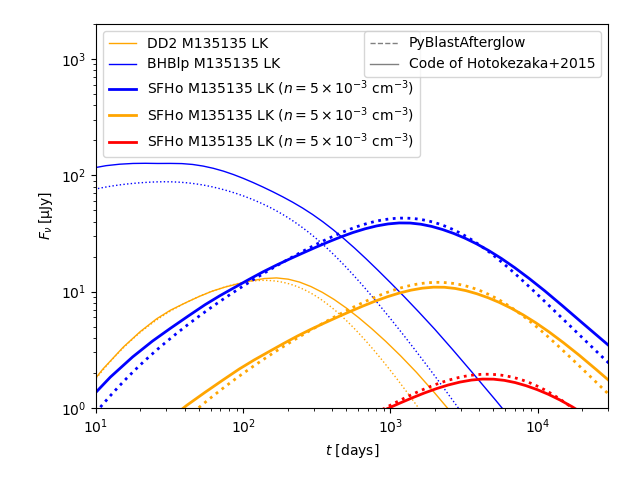
\includegraphics[width=0.49\textwidth]{ejecta_afterglow_vs_hotokezaka.png}
    \caption{
        Cumulative kinetic energy distribution for a selected set of models (\textit{top panel}) 
        and its angular distribution for a BLh $q=1.00$ model (\textit{bottom panel}).
        %% Also shown as a solid black line is the slow quasi-spherical model of \cite{Mooley:2017enz}.
        The vertical light green line marks the $\upsilon_{\text{ej}}=0.6$.
        The top panel shows that equal mass models have a more extend high energy tail,
        while the bottom panel shows that the angular distribution of the ejecta is not 
        uniform.
    } 
    \label{fig:afg_test}
\end{figure}

In Fig.~\ref{fig:afg_test} we show the \ac{kN} afterglow \acp{LC} from 
Figure~$30$ and Figure~$31$ of \citet{Radice:2018pdn}. The plot shows that that 
two codes are in a good agreement. The discrepancies observed can be attributed 
for different physical treatment of the \blast{} dynamics and synchrotron radiation. 
Notably, considering the large uncertainties on microphysical parameters and 
ejecta properties (discussed below) these discrepancies can be neglected.



\section{\ac{kN} afterglow for \GRB{} rebrightening} \label{sec:afterglow:results}


%Fig.~\ref{fig:ejecta_vel_hist}. 
%Notably, since the largest part (in mass) of the ejecta is equatorial it eludes the 
%interaction with the \ac{GRB} collimated ejecta and expands into an unshocked \ac{ISM}.
%The latter can decrease the \ac{ISM} density and delay the peak of the 
%synchotron emission \citep{2020MNRAS.495.4981M}.
%\red{move that to afterglow and rephrase}



\begin{figure*}%%[t]
    \centering 
    %% ---\includegraphics[width=0.49\textwidth]{./figs/scatter_lightcurve_peaks.pdf}
    %% \includegraphics[width=0.48\textwidth]{./figs/xray_obs_representative_all_eos.pdf}
    %% \includegraphics[width=0.48\textwidth]{./figs/radio_obs_representative_all_eos.pdf}
    %% --- \includegraphics[width=0.49\textwidth]{./figs/scatter_q_lam_ideaplot.pdf}
    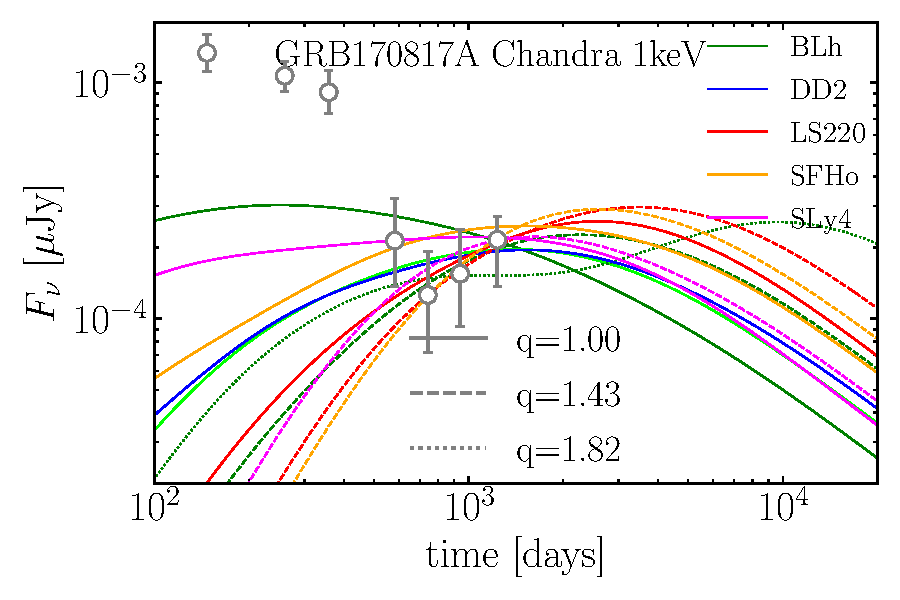
\includegraphics[width=0.48\textwidth]{kn_afterglow/best_xray_obs_representative_all_eos.pdf}
    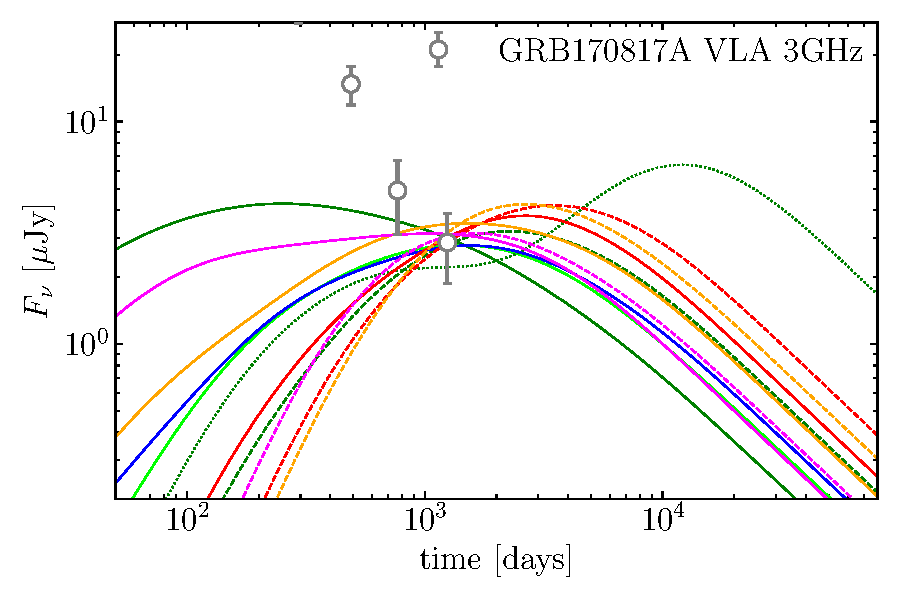
\includegraphics[width=0.48\textwidth]{kn_afterglow/best_radio_obs_representative_all_eos.pdf}
    \caption{
        Representative kilonova afterglow \acp{LC} for \ac{NR} models, 
        in X-ray (\textit{left panel}) and in radio (\textit{right panel}), where 
        %% There, every marker is annotated with two numbers, the tops is the peak time in years and the bottom is the peak flux in nJy ($10^{-9}$~Jy). The red color means that the value is below latest observations, that are $t=3.31$~years and $F_{\nu}=0.34$~$n$Jy. And the green color means that the model peak values are above the observational lower limit. 
        the gray circles are the observational data from \citet{Hajela:2021faz,Balasubramanian:2021kny}.
        %% The gray circles are the observational  in the X-ray band $0.3-10$~keV obtained from \citet{Fong:2017ekk,Hajela:2019mjy,Hajela:2020}.
        The synthetic \acp{LC} are computed with varying 
        micrphysical parameters and \ac{ISM} density within the 
        range of credibility to achieve a better fit to observational data (see Tab.~\ref{tab:pars} for details).
        %% The synthetic \acp{LC} are computed with the following parameters: 
        %% $\epsilon_e = 0.1$, $\epsilon_B\in(10^{-3},10^{-2})$, $n_{\text{ISM}}\in(10^{-3},10^{-2})$~$\ccm{}$.
        %% The last two parameters are varied for each model to achieve a better fit to the data. 
        %% ---
        The plots show that, within allowed parameter ranges, the \acp{LC} 
        from all models are in agreement with observations. 
        Models with moderately stiff \ac{EOS} and $q<1<1.8$ are tentatively preferred,
        as their flux is rising at $t\geq10^3$~days, in agreement with observations.
        %% --- 
        %% The plot shows that while for all models the peak time and magnitude are
        %% relatively close to the X-ray observed data, the models with moderately stiff \ac{EOS} and $q<1<1.8$ are tentatively preferred. 
    } 
    \label{fig:lightcurves}
\end{figure*}

\begin{table}
    \begin{center}
        \caption{
            List of parameters for synthetic \acp{LC} shown in the Fig~\ref{fig:lightcurves} 
            and Fig.~\ref{fig:lightcurve_peaks}.
            For the former the microphysical and \ac{ISM} density are adjusted model-wise 
            to achieved the good agreement with observations. For the latter,
            (the last row of the table) the parameters are the same for all models shown.
            Other parameters, such as observational angle, are the same everywhere (see text).
            (Adapted from \citet{Nedora:2021eoj})
        } \label{tab:pars}
        \scalebox{0.70}{
            \begin{tabular}{l | l l l l}
                Fig~\ref{fig:lightcurves} & $p$ & $\epsilon_e$ & $\epsilon_b$ & $n_{\text{ISM}}$ \\ \hline 
                BLh q=1.00    & 2.05 & 0.1          & 0.002        & 0.005            \\
                BLh q=1.43    & 2.05 & 0.1          & 0.003        & 0.005            \\
                BLh q=1.82    & 2.05 & 0.1          & 0.01         & 0.01             \\
                DD2 q=1.00    & 2.05 & 0.1          & 0.005        & 0.005            \\
                LS220 q=1.00  & 2.05 & 0.1          & 0.01         & 0.005            \\
                LS220 q=1.43  & 2.05 & 0.1          & 0.001        & 0.005            \\
                SFHo q=1.00   & 2.05 & 0.1          & 0.001        & 0.004            \\
                SFHo q=1.43   & 2.05 & 0.1          & 0.01         & 0.005            \\
                SLy4 q=1.00   & 2.05 & 0.1          & 0.001        & 0.004            \\
                SLy4 q=1.43   & 2.05 & 0.1          & 0.004        & 0.005            \\ \hline
                Fig.~\ref{fig:lightcurve_peaks}  & 2.15 & 0.2         & 0.005        & 0.005           
            \end{tabular}
        }
    \end{center}
\end{table}

In order to compute the \ac{kN} afterglow \acp{LC}, several free parameters of the model
need to be set. Specifically, we consider the \ac{ISM} density to be uniform with 
$\nism\in(10^{-3}, 10^{-2})\,\ccm$ \citep{Hajela:2019mjy}. 
The observational angle, (the angle between the line of sight and the polar axis of the 
\ac{BNS} system) is set to $\theta_{\text{obs}}=30\,$deg \citep{TheLIGOScientific:2017qsa}.
The luminosity distance of NGC 4993, the host galaxy of \GW{} is  $41.3\times10^{6}\,$pc 
with the redshift $z=0.0099$ \citep{Hjorth:2017yza}.
%
The index of the electron energy distribution, $p$, and microphysical parameters are 
chosed based on the recent observations of \GRB{}, where the spectral evolution 
was detected \citep{Hajela:2021faz}.  
%(see however \citet{Troja:2021xsw}). 
%
We consider 
$\varepsilon_e\in(0.1, 0.2)$,
$\varepsilon_B\in(10^{-3}, 10^{-2})$, 
$p\in[2.05,2.15]$.

\begin{figure}
    \begin{center}
        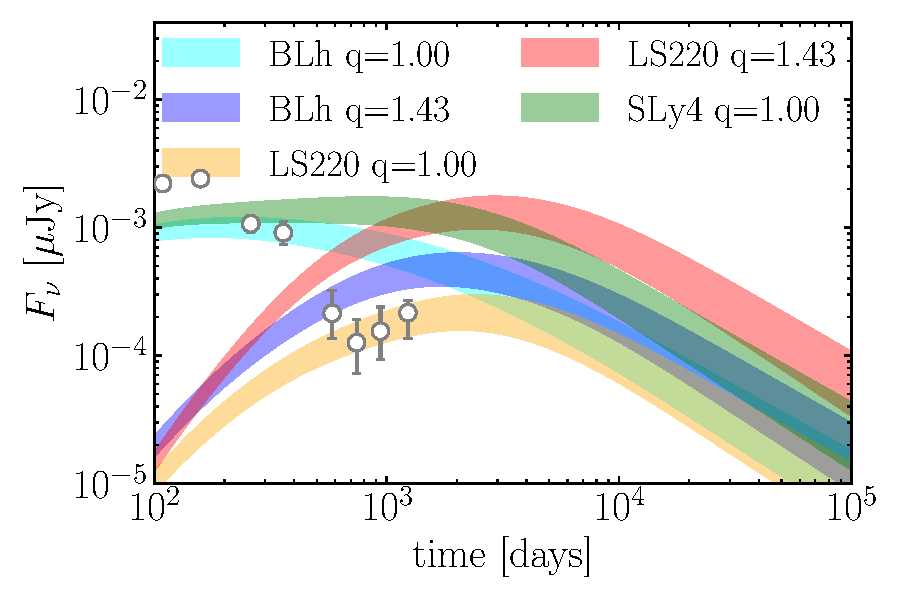
\includegraphics[scale=0.49]{kn_afterglow/KN-afterglow-NR-massratios.pdf}
        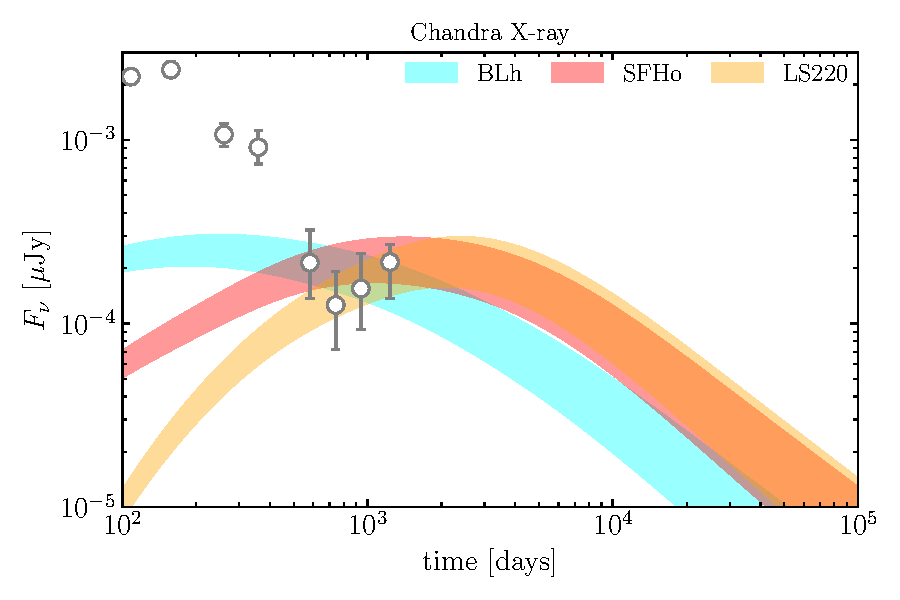
\includegraphics[scale=0.49]{kn_afterglow/KN-afterglow-NR-equalmass.pdf}
        \caption{
            The effect of the cahnging $p$ from $2.15$ (lower boundary of colored bands) to 
            $2.05$ (upper boundary of colored bands) shown in a set of \ac{kN} afterglow 
            X-ray \acp{LC} for \ac{DE} from a sample of \ac{NR} \ac{BNS} merger simulations.
            %% ---
            In \emph{upper panel} the models with different \mr{} are shown and the 
            $\nism=6\times10^{-3}$~cm$^{-3}$, and microphysical parameters, 
            $\varepsilon_{\rm e}=10^{-1}$, $\varepsilon_{\rm B}=10^{-2}$.
            %% --- 
            In \emph{lower panel} the models with $q=1$ are shown and afterglow
            parameters are adjusted to fit observations, 
            with $\varepsilon_{\rm e}=0.1$ fixed and  
            $\nism\sim 6\times 10^{-3}, 5\times 10^{-3},5\times 10^{-3}\,\rm{cm^{-3}}$
            $\varepsilon_{\rm B}\sim 10^{-2},2\times 10^{-3},10^{-3}$ for models with 
            LS220, BLh and SFHo \acp{EOS} respectively.
            (Adapted from \citet{Hajela:2021faz})\red{rephrased}
        } \label{fig:kn_afterglow}
    \end{center}
\end{figure}

Fig.~\ref{fig:lightcurves} shows the \acp{LC} in X-ray and radio bands for several 
representative \ac{BNS} merger models together with latest \GRB{} observational data. 
%% --- lightcurve shape
We observe, that ejecta velocity and angular distribution defines primarily the shape of the \acp{LC}.
Specifically, broad velocity distribution (found in equal mass \ac{BNS} models 
with soft \ac{EOS}, \eg, SLy4 \ac{EOS}) as shown in Fig.~\ref{fig:ejecta_vel_hist} 
translates into wide \acp{LC}, with an early rise time, comaptible with that of the early \GRB{} afterglow. 
This behaviour is guverned by the deceleration of the fastest ejecta shells, 
emission from which peak early. If the velocity distribution is rather narrow, with most of the 
material moving at ${\leq}0.2$~c (such is the model with LS220 \ac{EOS} and $q=1.43$) 
the \ac{LC} rise is steeper and occurs later (${\sim}10^2$~days after merger). 

%% --- general agreement with observations
Notably, the \ac{kN} afterglow \acp{LC} computed for most of our \ac{BNS} merger 
models are in good agreement with the 
rebrightening of the \GRB{} within the uncertainty introduced by microphsical 
parameters and \ac{ISM} density.
Specifically, this agreement is particularly good for models with moderately stiff 
\acp{EOS} and $1.00<q<1.82$, with respect to the \ac{LC} peak time.


From the \GRB{} model fitting the electron power law index $p$ is well constrain to $p=2.15$
\citep[\eg][]{Hajela:2019mjy}. The new emergent comonent in \GRB{} was found to have a lower 
$p=2.05$ \citep{Hajela:2021faz}. The effect of the decrease in $p$ is shown in 
Fig.~\ref{fig:kn_afterglow}. Notably, the parameters $p$, $\varepsilon_e$. $\varepsilon_b$ and 
$\nism$ are very degenerate, meaining that the change of one can be offset by the change in 
another withing these parameters' ranges of credibility inferred for \GRB{}. 

\begin{figure}%%[t]
    \centering 
    %%     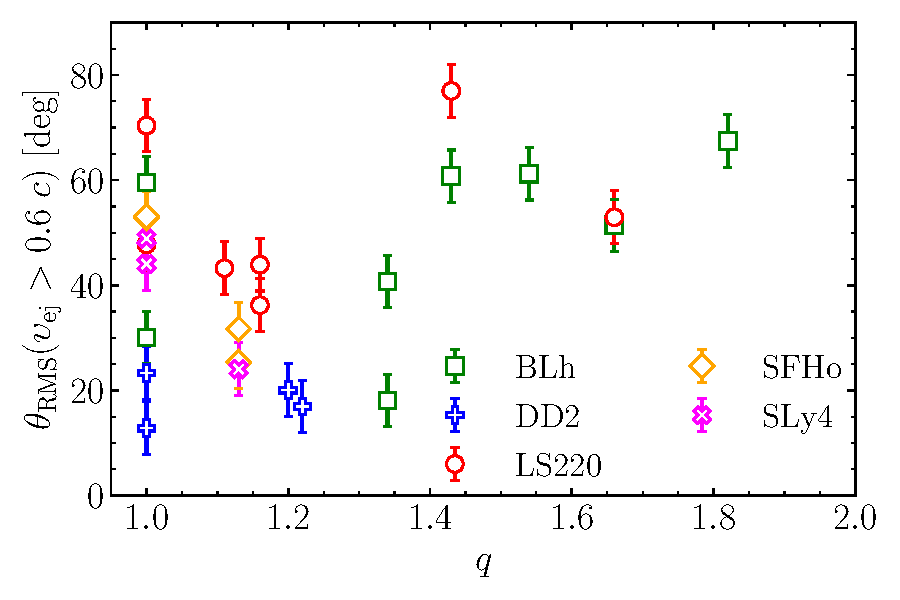
\includegraphics[width=0.49\textwidth]{./figs/scatter_thetarms_vej06.pdf}
    %% \includegraphics[width=0.49\textwidth]{figs/scatter_lightcurve_peaks_vs_lambda.pdf}
    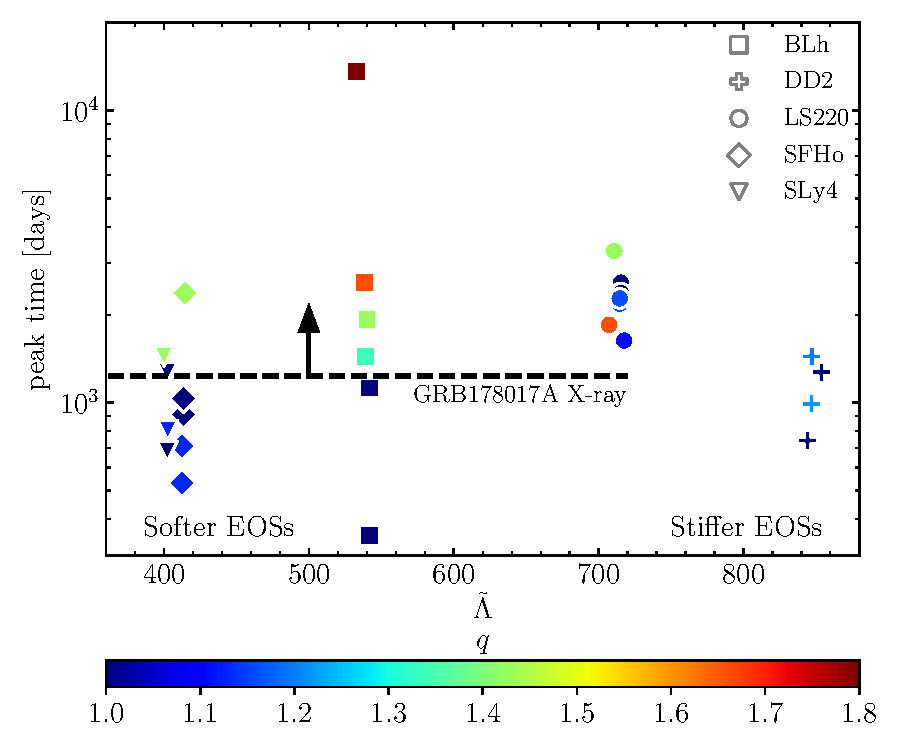
\includegraphics[width=0.49\textwidth]{kn_afterglow/scatter_lightcurve_tpeak_vs_lambda.pdf}
    \caption{
        Peak time, $t_p$, for \ac{LC} for all considered \ac{NR} simulations. 
        Dashed black line corresponds to the last observation of \GRB{} afterglow,
        where the rising flux implies that it is a lower limit on the kilonova 
        afterglow.
        The microphysical parameters and \ac{ISM} density for all models are fixed and 
        given in the Tab.~\ref{tab:pars}.
        The plot shows that in general the $t_p$ increases with mass ration and with 
        softness of the \ac{EOS}, except for the softest, DD2 \ac{EOS}. 
    } 
    \label{fig:lightcurve_peaks}
\end{figure}

%% --- Peak FLUX --- [UPDATED] --- IN CASE IT IS NEEDED [ BUT WITH NO FIGURE ]
If we fix the \ac{ISM} density and microphysical parameters to 
$\nism=5\times10^{-3}$~\gcm, $\varepsilon_e=0.1$ and $\varepsilon_b=5\times10^{-3}$, 
we observe that the \ac{LC} peak flux, $F_{\nu;p}\,$, is the highest for 
for models with soft \acp{EOS} such as SLy4. 
In general, however, we do not find a strong dependency between the \ac{EOS} and $F_{\nu;p}$.
With respect to the \mr{} we find that for models with stiff \acp{EOS}, 
the larger the \mr{}, the smaller is the $F_{\nu;p}$. 
%
This behaviour can be attributed to the overall dependency of the ejecta mass-averaged 
velocity on the \mr{} (see Fig.~\ref{fig:ejecta:dyn:dsfits}).
As the mass-averaged velocity decreases when \mr{} increases, the 
kinetic energy budget of the fast ejecta of these models decreases. 
Slower, more massive ejecta have lower peak flux.
Notably, for the models with stiffer \acp{EOS} the dependency on \mr{} is not clear. 

%% --- UNCERTANTIES --- dominant --- microphysics 
%% It is however important to note that the \ac{LC} fluxes and the $F_{\nu,p}$ 
%% depend strongly on the shock michrophsyics. Within the error bars provided by 
%% \citet{Hajela:2019mjy}, they can vary by more then one order of magnitude.  
%% Additionally, the slope of the electron distribution, 
%% $p$, was shown to be lower for the emerging new component of \GRB{} afterglow 
%% (Hajela et al.~in prep). The change from $p=2.15$ to $p=2.05$ translates to the
%% inclrease in $F_{\nu,p}$ by $\sim2$.
%% --- uncertanties -- subdominat -- ejecta
We find that the the \ac{LC} shape and peak time do not depend strongly on the 
uncertain microphysical parameters and \ac{ISM} density. With respect to the latter, 
the peak time changes by a facter of a few when $\nism\in(10^{-3},10^{-2})\,\ccm$.
Finite resolution effects that are present in ejecta properties do affect the 
afterglow \acp{LC}. Specifically, the $t_p$ changes by a factor of 
${\leq2}$, and $F_{\nu;p}$ changes withing a factor of ${\leq4}$. However, 
our analysis shows that the uncertainty in $\nism,\,\varepsilon_e,\,\varepsilon_b$ and $p$ are larger. 
%% --- Robust feature
%% Specifically, the \ac{LC} shape and the peak time appear to be robust 
%% both with resolution and with microphysics, as they set by the dynamics 

%\section{Discussion}
%
%In this section we considered the synchrotron afterglow arising from the interaction 
%of \ac{DE} and \ac{ISM} for a set of \ac{NR} \ac{BNS} models. 
%%
%The recent observations of \GRB{} by Chandra, ${\sim}10^3$~days after the \GW{} event 
%showed the emergence of the rising flux component. Our analysis suggests that this 
%rebrightening can be attributed to the emergence of the \ac{kN} afterglow, as its 
%properties, such as time and flux are naturally reproduced by the \ac{kN} afterglow 
%from ab-initio \ac{NR} \ac{BNS} simulations.
%%
%In the analysis we evolved the \ac{DE} with semi-analytic code and computed its 
%synchrotron emission. 
%We found that the synthetic \acp{LC} are in agreement with the emerging new component 
%in the \GRB{} afterglow within the range of credibility of the microphisycal parameters 
%and of the \ac{ISM} density, $n_{\text{ISM}}$. 
%% The \ac{LC} shape and the time of the peak depends primarily on the 
%% ejecta velocity distribution. If massive fast ejecta component is present, the \ac{LC} 
%% is broader and peaks before $10^3$~days postmerger, while afterglow from 
%% the ejecta with small/absent fast tail peaks on the timescale of $>10^3$~days 
%% (see Fig.\ref{fig:lightcurves}). 

%% --- Note on the observations
%% The latest \GRB{} observations by Chandra \newtxt{(and possibly VLA)} 
%% at $1234$~days show a rising flux (Hajela \textit{et al.} (in prep.)). 

Comparing the \GRB{} observations and synthetic \acp{LC} we observe, that the 
rebrightening at $1243$~days after merger has the following implications:
the \ac{kN} afterglow peak should be (i) later and (ii) brighter than what is
currently observed. 
%
The condition (ii) is weak as the \ac{LC} peak flux is not well constrained due to 
uncertain microphysical parameters.
%% With respect to our models, the (ii) condition suggests that models soft \ac{EOS} and large \mr{} are disfavoured, 
%% as their $F_{\nu,p}$ is lower then the observations.
%% However, an increase in $\epsilon_B$ by a factor of $2$ changes this result.
The condition (i), however, is more robust from that point of view and allows to 
asses, afterglow from which models is more supported by observations.

%% --- PEAK TIME 
We show the peak time of the afterglow \acp{LC} of all our models in 
Fig.~\ref{fig:lightcurve_peaks}. There, the microphysical parameters and $\nism$ are fixed 
and listed in Tab.~\ref{tab:pars}, last row). 
We consider all models here, including those that do not have fast ejecta tail 
(see Sec.~\ref{sec:bns_sims:fast_de}) as their ejecta is still energetic enough 
to produce bright afterglow. 
%
The \ac{LC} peak times are ${\sim}10^3$~days for all models that do not undergo the 
tidal disruption. The latter, (BLh $q=1.82$ (\texttt{SR}) model) produces massive and 
slow ejecta that is characterized by the late afterglow \ac{LC} peak 
of ${\sim}10^4\,$days.
%
Overall, we observe that the $t_{p}<10^3$~days for models with $q\sim1$ and 
$t_p>10^3$~days for models with larger \mr{}. This relation appears more prominent for 
models with soft \acp{EOS}, as the ejecta in these models has a strong contribution from 
shocked, fast component of \ac{DE} (when \mr{} is small), and the 
kinetic energy of the ejecta fast tail increases with the contribution from the 
shocked component (see Fig.~\ref{fig:ejecta_v06}). 
And the afterglow of faster, less massive ejecta peaks earlier 
\citep[\eg][]{Hotokezaka:2015eja}.
Indeed, the time of the \ac{LC} peak depends primarily on the ejecta 
dynamics, the so-called deceleration time \citep[\eg][]{Piran:2012wd}.
%% --- 
%% In the Fig.~\ref{fig:lightcurve_peaks} we show the peak time, $t_{p}$, for each model, 
%% alongside the lower limit (the time of the latest observation).
%% --- 
In Fig.~\ref{fig:lightcurve_peaks} we also show the time of the latest observation 
of the rising flux in \GRB{} (horizontal line). This provides the lower limit on $t_p$
in accordance with (ii).
%
We observe that the synthetic \acp{LC} of models with 
moderate amount of fast ejecta, \eg, models with 
\acp{EOS} of mild stiffness and \mr{}, lie above the limit, while models with very 
energetic fast tails, found $q=1$ models with very stiff \acp{EOS}, peak earlier. 
%% ---

%%%% <<< moved to overall conclusion >>>
%The main conclusion of our work is that the observed rising flux in the afterglow of \GRB{} 
%at $10^3$~days can be explained by the \ac{kN} afterglow produced by ejecta in 
%ab-initio \ac{NR} \ac{BNS} simulations targeted to \GW{}. 
%%% ---
%Specifically, models with moderately stiff \acp{EOS} and moderately large \mr{}, 
%that produce a mild amount of fast ejecta, are favored.
%%% ---
%Out results are subjected to uncertainties, the dominant among which are introduced 
%by ill-constrained microphysical parameters. 
% Additionally, the systematic effects due to the finite resolution, neutrino treatment 
%and \acp{EOS} might be important. 
%%% ---
%A larger set of observations, that allows for a better assessment of shock microphysics, 
%and a larger sample of high resolution \ac{NR} simulations are required to investigate 
%these uncertainties further. We leave this to future works.